\startcontents[localtoc]
\printcontents[localtoc]{}{0}{\section*{Contents}\setcounter{tocdepth}{2}}



\phantomsection
\addcontentsline{toc}{section}{Overview}
\subsection*{Overview}



A function qwtbvar\_example\_1\_process() calculating hyperparaboloid is used to
demonstrate the QWBTvar. Input quantities will be varied to calculate outputs
for multiple series of inputs.



\phantomsection
\addcontentsline{toc}{section}{Inputs}
\subsection*{Inputs}



Input quantities:

\begin{lstlisting}
DI.x.v = 0;
DI.y.v = 0;
DI.a.v = 1;
DI.a.u = 0;
DI.b.v = 2;
\end{lstlisting}


Varied input quantities:

\begin{lstlisting}
DIvar.a.v = [1 2];
DIvar.a.u = [0 0.25 0.5];
DIvar.x.v = [-5  -2   0   2   5];
DIvar.y.v = [-5; -3; -1;  1;  3;  5];
\end{lstlisting}


Some optional settings:

\begin{lstlisting}
CS.verbose = 1;
CS.mcm.repeats = 1e3;
CS.var.dir = 'qwtbvar_example_1_calculation_data';
CS.var.cleanfiles = 1;
CS.var.method = 'singlecore';
CS.var.procno = 1;
\end{lstlisting}


\phantomsection
\addcontentsline{toc}{section}{Calculation}
\subsection*{Calculation}



Run whole calculation. Input quantities in DI will be varied according DIvar:

\begin{lstlisting}
[jobfn] = qwtbvar('calc', 'qwtbvar_example_1_process', DI, DIvar, CS);
\end{lstlisting}
\begin{lstlisting}[language={},xleftmargin=5pt,frame=none]
### QWTBVAR: Number of variation calculations is: 180
### QWTBVAR: All calculations finished. The calculations took 0.0573 s (0.000956 m, 1.59e-05 h)

\end{lstlisting}


\phantomsection
\addcontentsline{toc}{section}{Plotting}
\subsection*{Plotting}



Plot results. Results are multidimensional. To plot 3D or 2D plots, the consts
will contain 'constant' values that will be used to select data from
multidimensional results to decrease dimensions and simplify plotting:

\begin{lstlisting}
consts.a.v = 1;
consts.a.u = 0.25;
\end{lstlisting}


3 dimensional plot:

\begin{lstlisting}
qwtbvar('plot3D', jobfn, 'x', 'y', 'z', consts);
\end{lstlisting}
\begin{center}
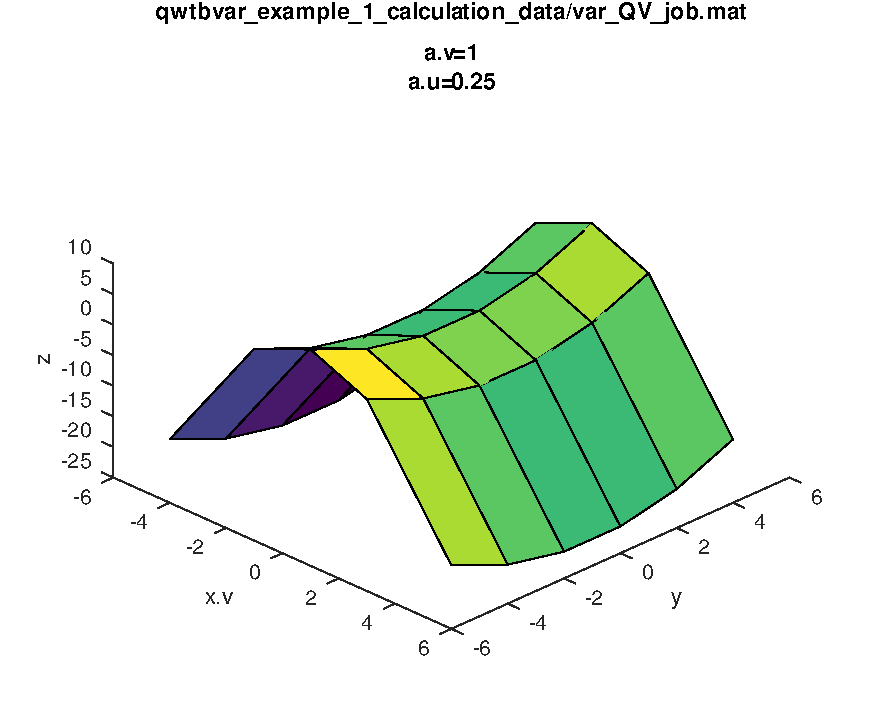
\includegraphics[width=0.7\textwidth]{qwtb_examples_published/qwtbvar_example_1-1.pdf}
\end{center}


Add another constant to plot simple 2 dimensional figure:

\begin{lstlisting}
consts.y.v = 1;
qwtbvar('plot2D', jobfn, 'x', 'z', consts);
\end{lstlisting}
\begin{center}
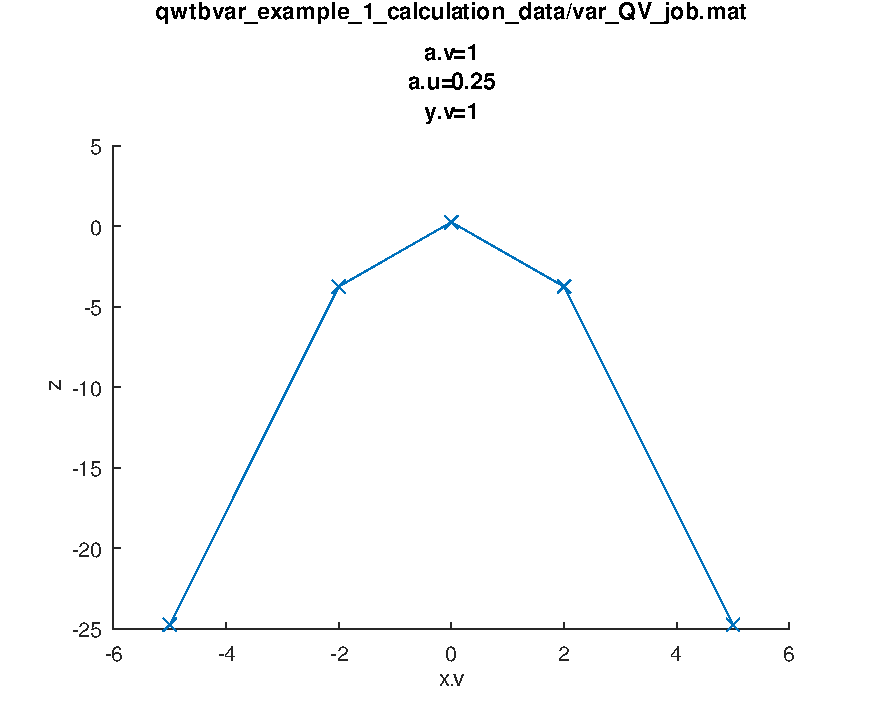
\includegraphics[width=0.7\textwidth]{qwtb_examples_published/qwtbvar_example_1-2.pdf}
\end{center}


\phantomsection
\addcontentsline{toc}{section}{Look Up Table}
\subsection*{Look Up Table}



Set up additional information for axes of the multidimensional results that
will be used to create look-up table.

\begin{lstlisting}
axset.a.v.min_ovr = min(DIvar.a.v)-0.1;
axset.a.v.max_ovr = max(DIvar.a.v)+0.1;
axset.a.v.min_lim = 'error';
axset.a.v.max_lim = 'error';
axset.a.v.scale = 'lin';
axset.a.u.min_ovr = min(DIvar.a.u);
axset.a.u.max_ovr = max(DIvar.a.u);
axset.a.u.min_lim = 'error';
axset.a.u.max_lim = 'error';
axset.a.u.scale = 'lin';
axset.x.v.min_ovr = min(DIvar.x.v)-3;
axset.x.v.max_ovr = max(DIvar.x.v)+3;
axset.x.v.min_lim = 'const';
axset.x.v.max_lim = 'const';
axset.x.v.scale = 'lin';
axset.y.v.min_ovr = min(DIvar.y.v)-3;
axset.y.v.max_ovr = max(DIvar.y.v)+3;
axset.y.v.min_lim = 'const';
axset.y.v.max_lim = 'const';
axset.y.v.scale = 'lin';
\end{lstlisting}


Set type of scaling for output quantity.

\begin{lstlisting}
rqset.z.v.scale = 'lin';
\end{lstlisting}


Create look up table that will be used for interpolation.

\begin{lstlisting}
lut = qwtbvar('lut', jobfn, axset, rqset);
\end{lstlisting}


\phantomsection
\addcontentsline{toc}{section}{Interpolation of results}
\subsection*{Interpolation of results}



Set parameters for interpolation:

\begin{lstlisting}
ipoint.a.v = 1.5;
ipoint.a.u = 0;
ipoint.x.v = 0;
ipoint.y.v = 0;
\end{lstlisting}


Create a range of input quantities for which the interpolation will be done:

\begin{lstlisting}
x = -7:0.5:7;
y = -7:0.5:7;
% For all input quantities values, interpolate:
for j = 1:numel(x)
    ipoint.x.v = x(j);
    for k = 1:numel(y)
        ipoint.y.v = y(k);
        tmp = qwtbvar('interp', lut, ipoint);
        ival(j, k) = tmp.z.v;
    end
end
\end{lstlisting}


Plot figure with interpolated values based on the LUT:

\begin{lstlisting}
figure
mesh(ival)
title('Interpolated values of z.v, based on LUT')
xlabel = 'x.v';
ylabel = 'y.v';
\end{lstlisting}
\begin{center}
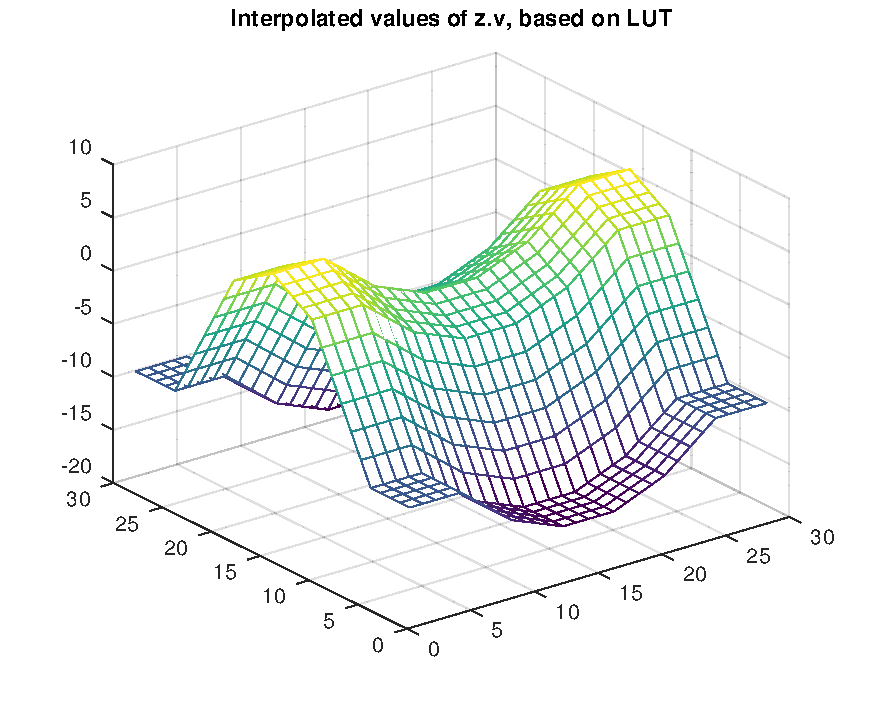
\includegraphics[width=0.7\textwidth]{qwtb_examples_published/qwtbvar_example_1-3.pdf}
\end{center}


\stopcontents[localtoc]
